\documentclass[
  twocolumn,
  aps,
  pra,
  floatfix,
  amsmath,amssymb,
  longbibliography
]{revtex4-2}

\usepackage[T1]{fontenc}
\usepackage[utf8]{inputenc}
\usepackage{amsthm}
\usepackage{graphicx}
\usepackage{xcolor}
\usepackage{tikz}
\usetikzlibrary{arrows.meta}
\usepackage[
  breaklinks=true,
  colorlinks=true,
  citecolor=blue,
  linkcolor=blue,
  urlcolor=blue
]{hyperref}
\usepackage{orcidlink}
\hypersetup{
  pdftitle={Different Quantum Descriptions, Identical Statistics},
  pdfauthor={Mirko Navara and Karl Svozil},
  pdfkeywords={quantum pseudocontext, rank-one decomposition, frame operator,
    Bloch sphere, tight frame, positive operator-valued measure}
}

\newtheorem{theorem}{Theorem}
\newtheorem{lemma}[theorem]{Lemma}
\newtheorem{proposition}[theorem]{Proposition}
\newtheorem{corollary}[theorem]{Corollary}

\theoremstyle{definition}
\newtheorem{definition}[theorem]{Definition}
\newtheorem{example}[theorem]{Example}

\theoremstyle{remark}
\newtheorem{remark}[theorem]{Remark}
\newtheorem{problem}[theorem]{Open Problem}

\newcommand{\R}{\mathbb R}
\newcommand{\C}{\mathbb C}
\newcommand{\F}{\mathbb F}
\newcommand{\supp}{\operatorname{supp}}
\newcommand{\ran}{\operatorname{ran}}
\newcommand{\diag}{\operatorname{diag}}
\newcommand{\Tr}{\operatorname{tr}}
\newcommand{\1}{\mathbf 1}

\begin{document}

\title{Different Quantum Descriptions, Identical Statistics}

\author{Mirko Navara\,\orcidlink{0000-0002-0880-5992}}
\affiliation{Faculty of Electrical Engineering, Czech Technical University in Prague,
Technick\'{a} 2, CZ-166~27 Prague 6, Czech Republic}
\email{navara@fel.cvut.cz}

\author{Karl Svozil\,\orcidlink{0000-0001-6554-2802}}
\affiliation{Institute for Theoretical Physics, TU Wien,
Wiedner Hauptstrasse 8-10/136, A-1040 Vienna, Austria}
\email{karl.svozil@tuwien.ac.at}

\date{\today}

\begin{abstract}
We introduce quantum pseudocontexts: two separate collections of quantum
alternatives that, although assembled differently, give the same total
probability for every possible state.  This agreement belongs to the chosen
quantum description and need not follow from the bare pattern of which
alternatives exclude one another.  We identify when such examples are
genuinely different from ordinary complete measurements, show that allowing
phases makes smaller examples possible, and give broad families of examples.
The same idea also describes two randomized preparation procedures that cannot
be distinguished once their labels are forgotten, or two measurements that
agree after selected outcomes are grouped together.
\end{abstract}

\maketitle

% ------------------------------------------------------------------
\section{Introduction}
% ------------------------------------------------------------------

Let $a_1,\ldots,a_k$ and $b_1,\ldots,b_k$ be rays in a finite-dimensional
real or complex Hilbert space.  The identity
\begin{equation}
 \sum_{i=1}^{k}P_{a_i}=\sum_{i=1}^{k}P_{b_i}
 \label{eq:intro-operator}
\end{equation}
between their rank-one projectors implies
\begin{equation}
 \sum_{i=1}^{k}\Tr(\rho P_{a_i})
 =\sum_{i=1}^{k}\Tr(\rho P_{b_i})
 \label{eq:intro-probability}
\end{equation}
for every density operator $\rho$.  The two collections need not be
orthogonal, jointly measurable, or bases.  They are two different quantum
descriptions of the same positive operator.

Families with this property arose in the study of probabilistic equivalence
between noncommuting observables~\cite{2023-navara-svozil,NSvozil:QS24}.  Two
notions should now be separated.  In the stronger, combinatorial notion, a
finite set of context-normalization equations forces the equality,
independently of a faithful orthogonal representation and of the probability theory
\cite{2026-Navara-Svozil-pseudocontexts}.  The present paper studies
the weaker quantum notion in Eq.~\eqref{eq:intro-operator}.  The coordinates,
or equivalently the projectors, are part of the data.  The equality is
universal over Born-rule states for those data but need not hold after a
recoordinatization or for classical, softmax-generated, or other probability
assignments.

This weaker notion has its own natural theory.  It is a problem about equal
unit-norm rank-one decompositions, hence about finite frames and positive
operators.  We establish the sharp minimum genuine sizes over $\R$ and $\C$,
give continuous constructions for every allowed size, describe the complete
two-dimensional geometry, and organize the general case by the spectrum and
commutant of the common operator.  A four-ray example will also show directly
that quantum equality alone does not imply hypergraph or classical equality.

% ------------------------------------------------------------------
\section{Definition and operator equivalence}
\label{sec:definition}
% ------------------------------------------------------------------

Throughout, $\F\in\{\R,\C\}$ and $H$ is a finite-dimensional Hilbert space
over $\F$.  For a nonzero vector $v\in H$, we write
\[
 [v]:=\operatorname{span}\{v\}=\F v
     =\{\alpha v:\alpha\in\F\}
\]
for the ray, that is, the one-dimensional linear subspace, spanned by $v$.
The orthogonal projector onto this ray is
\begin{equation}
 P_v=\frac{|v\rangle\langle v|}{\langle v,v\rangle}.
 \label{eq:ray-projector}
\end{equation}
Thus $P_v$ depends only on the ray $[v]$.  For a density operator $\rho$, the Born
probability of this ray is
\begin{equation}
 p_\rho(v)=\Tr(\rho P_v),\qquad \rho\ge0,\quad\Tr\rho=1.
 \label{eq:born}
\end{equation}
In dimension at least three these are precisely the finitely additive
Hilbert-lattice states under the hypotheses of Gleason's theorem
\cite{Gleason}.  In dimension two we deliberately restrict attention to
density-operator states.

\begin{lemma}[Separation by quantum states]
\label{lem:separation}
If self-adjoint operators $X,Y$ satisfy
$\Tr(\rho X)=\Tr(\rho Y)$ for every density operator $\rho$, then $X=Y$.
\end{lemma}

\begin{proof}
Set $C=X-Y$.  Since both $X$ and $Y$ are self-adjoint, so is $C$.  Let $x$
be any unit vector.  The rank-one projector $P_x$ is positive and has trace
one, so it is a density operator.  The hypothesis of the lemma therefore
gives
\[
 0=\Tr(P_xX)-\Tr(P_xY)=\Tr(P_xC)=\langle x,Cx\rangle.
\]
Thus the expectation value of $C$ vanishes in every pure state.

Suppose, for contradiction, that $C\ne0$.  By the finite-dimensional
spectral theorem, a nonzero self-adjoint operator has a nonzero real
eigenvalue $\mu$ and a corresponding unit eigenvector $u$.  Hence
\[
 0=\langle u,Cu\rangle
  =\langle u,\mu u\rangle
  =\mu\|u\|^2
  =\mu,
\]
contrary to $\mu\ne0$.  Therefore $C=0$, and consequently $X=Y$.
\end{proof}

\begin{definition}[Quantum pseudocontext]
\label{def:quantum-pseudocontext}
A \emph{quantum pseudocontext of size $k$} in $H$ is a pair of $k$-element
ray families
\[
 A=\{[a_1],\ldots,[a_k]\},\qquad
 B=\{[b_1],\ldots,[b_k]\}
\]
where $a_i$ and $b_i$ are chosen unit representatives of their respective
rays.  This normalization does not affect the projectors or Born
probabilities, which depend only on the rays.  The rays within each family
are required to be distinct, $A\cap B=\varnothing$, and
\begin{equation}
 \sum_{i=1}^{k}p_\rho(a_i)=\sum_{i=1}^{k}p_\rho(b_i)
 \quad\text{for every density operator }\rho.
 \label{eq:def-probability}
\end{equation}
It is \emph{genuine} if neither family is an orthonormal basis of its
supporting subspace.
\end{definition}

Disjointness prevents trivial padding by rays common to both sides.  An
orthonormal basis of the common support will be called a relative context; it
need not be a basis of the ambient Hilbert space.

By Lemma~\ref{lem:separation}, Definition~\ref{def:quantum-pseudocontext} is
equivalent to Eq.~\eqref{eq:intro-operator}.  The common positive operator
\begin{equation}
 T:=\sum_{i=1}^{k}P_{a_i}=\sum_{i=1}^{k}P_{b_i}
 \label{eq:structure}
\end{equation}
is the common frame operator of the two families; we call it the
\emph{structure operator}.  In particular,
\begin{equation}
 T\ge0,\qquad \Tr T=k,\qquad \operatorname{rank}T\le k.
 \label{eq:basic-T}
\end{equation}

\begin{proposition}[Genuineness criterion]
\label{prop:genuine}
For a quantum pseudocontext with structure operator $T$, write
$\ran T:=\{Tx:x\in H\}$ for the range of $T$, and let
$\lambda_{\max}(T)$ denote the largest eigenvalue of $T$.  Then the following
are equivalent:
\begin{enumerate}
 \item the pseudocontext is genuine;
 \item $T$ is not the orthogonal projector onto $\ran T$;
 \item $\lambda_{\max}(T)>1$.
\end{enumerate}
\end{proposition}

\begin{proof}
We first identify the subspace $\ran T$.  For every $x\in H$,
\[
 \langle x,Tx\rangle
 =\sum_{i=1}^{k}|\langle a_i,x\rangle|^2.
\]
Consequently, $Tx=0$ exactly when $x$ is orthogonal to every $a_i$.  Thus
\[
 \ker T=\operatorname{span}\{a_1,\ldots,a_k\}^{\perp}.
\]
Since $T$ is self-adjoint, its range is the orthogonal complement of its
kernel.  Therefore
\[
 \ran T=\operatorname{span}\{a_1,\ldots,a_k\}.
\]
Using the second expression for $T$ in Eq.~\eqref{eq:structure} gives
similarly
\[
 \ran T=\operatorname{span}\{b_1,\ldots,b_k\}.
\]
Hence $\ran T$ is the common supporting subspace of the two families.

Let $P_{\ran T}$ denote the orthogonal projector onto $\ran T$.  If the
$a_i$ form an orthonormal basis of $\ran T$, then the usual resolution of
the identity on this subspace gives
\[
 T=\sum_{i=1}^{k}P_{a_i}=P_{\ran T}.
\]
Conversely, suppose that $T=P_{\ran T}$.  Since every $a_j$ lies in
$\ran T$ and has unit norm,
\begin{align*}
 1
 &=\langle a_j,P_{\ran T}a_j\rangle
  =\langle a_j,Ta_j\rangle\\
 &=\sum_{i=1}^{k}|\langle a_i,a_j\rangle|^2
  =1+\sum_{i\ne j}|\langle a_i,a_j\rangle|^2.
\end{align*}
It follows that $\langle a_i,a_j\rangle=0$ whenever $i\ne j$.  The $a_i$
therefore form an orthonormal basis of their span, which is $\ran T$.
The same argument applies to the $b_i$.  Thus either both families are
orthonormal bases of their common support or neither family is.  By the
definition of genuineness, this proves the equivalence of (1) and (2).

It remains to relate (2) to the largest eigenvalue.  Put
$r=\operatorname{rank}T$, and denote the nonzero eigenvalues of $T$ by
$\lambda_1,\ldots,\lambda_r$.  They are positive because $T\ge0$.  If
$\lambda_{\max}(T)\le1$, then every $\lambda_j\le1$, and therefore
\[
 k=\Tr T=\sum_{j=1}^{r}\lambda_j\le r
   =\operatorname{rank}T\le k,
\]
where the first and last relations follow from Eq.~\eqref{eq:basic-T}.
Equality must hold throughout.  In particular, every nonzero eigenvalue of
$T$ equals one.  Hence $T$ acts as the identity on $\ran T$ and as zero on
its orthogonal complement, so $T=P_{\ran T}$.

Conversely, if $T=P_{\ran T}$, then all its nonzero eigenvalues equal one,
and therefore $\lambda_{\max}(T)=1$.  We have proved that
\[
 T\ne P_{\ran T}
 \quad\Longleftrightarrow\quad
 \lambda_{\max}(T)>1,
\]
which establishes the equivalence of (2) and (3).
\end{proof}

Consequently, a genuine quantum pseudocontext equates two Born-weight sums
that can exceed one.  The equality of the sums is state-independent; their
common numerical value $\Tr(\rho T)$ is generally state-dependent.  The
exceptional constant cases are characterized in
Proposition~\ref{prop:constancy}.

% ------------------------------------------------------------------
\section{Quantum equality need not be classically forced}
\label{sec:not-forced}
% ------------------------------------------------------------------

The smallest genuine complex example already shows that the quantum identity
is not imposed on arbitrary hypergraph-free probability assignments.

\begin{example}[A non-forced four-ray identity]
\label{ex:k2}
In $\C^2$, let
\begin{equation}
 u_\pm=\left(\frac{\sqrt3}{2},\,\pm\frac12\right),\qquad
 v_\pm=\left(\frac{\sqrt3}{2},\,\pm\frac{i}{2}\right).
 \label{eq:k2-vectors}
\end{equation}
The four rays are distinct and
\begin{equation}
 P_{u_+}+P_{u_-}=P_{v_+}+P_{v_-}
 =\diag\left(\frac32,\frac12\right).
 \label{eq:k2-identity}
\end{equation}
The inner product within each pair equals $1/2$, so the quantum
pseudocontext is genuine.
\end{example}

Every pair among the four rays is nonorthogonal: the cross inner products are
$3/4\pm i/4$.  Their bare orthogonality hypergraph therefore has no contexts
and imposes no normalization equation.  The assignment
\begin{equation}
 q(u_+)=q(u_-)=1,\qquad q(v_+)=q(v_-)=0
 \label{eq:classical-counterexample}
\end{equation}
is admissible under the bare-hypergraph convention, which imposes no
context-normalization constraints, yet
its two sums are $2$ and $0$.  A generic softmax or other parametrization can
likewise violate the equality.  Equation~\eqref{eq:k2-identity} is guaranteed
only when the probabilities are produced from the displayed projectors by
the Born rule, or by another model that separately imposes the same operator
identity.

This example also shows why quantifying over every density operator does not
make the identity coordinatization-independent.  Moving the four rays while
preserving their empty orthogonality graph will generically destroy
Eq.~\eqref{eq:k2-identity}.

% ------------------------------------------------------------------
\section{Dimension two: Bloch geometry and sharp thresholds}
\label{sec:bloch}
% ------------------------------------------------------------------

Every rank-one projector in $\C^2$ has the Bloch form
\begin{equation}
 P_a=\frac12\bigl(I+\boldsymbol r_a\boldsymbol\cdot\boldsymbol\sigma\bigr),
 \qquad \boldsymbol r_a\in S^2\subset\R^3,
 \label{eq:bloch}
\end{equation}
where $\boldsymbol\sigma$ denotes the Pauli vector.

\begin{theorem}[Bloch-sphere characterization]
\label{thm:bloch}
Two disjoint $k$-element ray families in $\C^2$ form a quantum
pseudocontext if and only if their Bloch vectors have the same sum:
\begin{equation}
 \sum_{i=1}^{k}\boldsymbol r_{a_i}
 =\sum_{i=1}^{k}\boldsymbol r_{b_i}.
 \label{eq:bloch-centroid}
\end{equation}
The structure operator is
\begin{equation}
 T=\frac{k}{2}I+\frac12\boldsymbol R\boldsymbol\cdot\boldsymbol\sigma,
 \qquad \boldsymbol R=\sum_i\boldsymbol r_{a_i},
 \label{eq:bloch-T}
\end{equation}
and has eigenvalues
\begin{equation}
 \lambda_\pm=\frac{k\pm\|\boldsymbol R\|}{2}.
 \label{eq:bloch-spectrum}
\end{equation}
\end{theorem}

\begin{proof}
Substitution of Eq.~\eqref{eq:bloch} into the two projector sums proves
Eq.~\eqref{eq:bloch-centroid}, because
$I,\sigma_x,\sigma_y,\sigma_z$ are linearly independent.  The Pauli identity
$(\boldsymbol R\boldsymbol\cdot\boldsymbol\sigma)^2=\|\boldsymbol R\|^2I$
gives the spectrum.
\end{proof}

For $k=2$ and $0<\|\boldsymbol R\|<2$, write
\begin{equation}
 \boldsymbol r_{1,2}=\frac{\boldsymbol R}{2}\pm\boldsymbol w,
 \qquad \boldsymbol w\perp\boldsymbol R,\quad
 \|\boldsymbol w\|^2=1-\frac{\|\boldsymbol R\|^2}{4}.
 \label{eq:bloch-circle}
\end{equation}
Thus the unordered two-point decompositions of a fixed nonzero
$\boldsymbol R$ form a circle.  Example~\ref{ex:k2} selects two points on
this circle of decompositions.

The real projective line is different.  A real ray represented by
$x_\theta=(\cos\theta,\sin\theta)$ has
\begin{equation}
 P_\theta=\frac12
 \begin{pmatrix}
 1+\cos2\theta&\sin2\theta\\
 \sin2\theta&1-\cos2\theta
 \end{pmatrix}.
 \label{eq:real-bloch}
\end{equation}
It is therefore represented by a point
$q_\theta=(\cos2\theta,\sin2\theta)$ on a circle rather than by the full
Bloch sphere.

\begin{proposition}[Real rigidity at size two]
\label{prop:real-k2}
No genuine quantum pseudocontext of size $k=2$ exists in a real
finite-dimensional Hilbert space.
\end{proposition}

\begin{proof}
The common range of two equal two-projector sums has dimension at most two,
and it cannot be one-dimensional: in a one-dimensional range all four
projectors would have the same ray, contrary to distinctness and
disjointness.  It is therefore enough to work in $\R^2$.  Equality is
equivalent, by Eq.~\eqref{eq:real-bloch}, to equality of two sums of unit
vectors on the doubled-angle circle.  If unit vectors $x,y$ satisfy
$x+y=s\ne0$, then
\[
 \begin{aligned}
 x&=\frac{s}{2}+w,& y&=\frac{s}{2}-w,\\
 w&\perp s,& \|w\|^2&=1-\frac{\|s\|^2}{4}.
 \end{aligned}
\]
In the plane, $w$ is determined up to sign, which only exchanges $x$ and
$y$.  Thus a nonzero vector has a unique decomposition into two unit circle
points, up to permutation, and the two ray pairs coincide.  If
the common doubled-angle vector sum is zero, each pair is antipodal on the
doubled-angle circle, which means that the original rays are orthogonal.  Both
pairs are then relative contexts and the construction is not genuine.
\end{proof}

The geometric reason is codimension: the complex Bloch sphere offers a circle
of chords with a fixed midpoint, while the real Bloch circle offers only one
such chord.

% ------------------------------------------------------------------
\section{Constructions of every allowed size}
\label{sec:all-sizes}
% ------------------------------------------------------------------

The complex size-two phase freedom extends uniformly to all sizes.

\begin{theorem}[Complex phase construction]
\label{thm:complex-phase}
Let $H$ contain an orthonormal pair $e_1,e_2$, let $k\ge2$, and put
$\omega=e^{2\pi i/k}$.  Choose $\alpha\in(0,\pi/2)$ and a phase $e^{i\phi}$
that is not a $k$th root of unity.  For $j=0,\ldots,k-1$, define
\begin{align}
 a_j&=\cos\alpha\,e_1+\sin\alpha\,\omega^j e_2,\nonumber\\
 b_j&=\cos\alpha\,e_1+\sin\alpha\,e^{i\phi}\omega^j e_2.
 \label{eq:phase-vectors}
\end{align}
Then all $2k$ rays are distinct and
\begin{equation}
 \sum_{j=0}^{k-1}P_{a_j}=\sum_{j=0}^{k-1}P_{b_j}
 =k\bigl(\cos^2\alpha\,P_{e_1}+\sin^2\alpha\,P_{e_2}\bigr).
 \label{eq:phase-T}
\end{equation}
The quantum pseudocontext is genuine whenever $k\ge3$, and also for $k=2$
provided $\alpha\ne\pi/4$.
\end{theorem}

\begin{proof}
In each projector, the diagonal terms are
$\cos^2\alpha\,P_{e_1}+\sin^2\alpha\,P_{e_2}$.  The off-diagonal terms are
proportional to $\omega^j$ or $\omega^{-j}$ and vanish upon summation because
$\sum_{j=0}^{k-1}\omega^j=0$.  The additional phase in the $b$-family does
not affect this cancellation.

Comparison of the nonzero $e_1$ components shows that two vectors in
Eq.~\eqref{eq:phase-vectors} can span the same ray only if their second
components agree.  Powers of $\omega$ distinguish rays within each family,
and the assumption on $e^{i\phi}$ excludes cross-family collisions.  For
$k\ge3$, a $k$-element family in a two-dimensional support cannot be a basis.
For $k=2$, the inner product within each pair is $\cos2\alpha$, which is
nonzero exactly when $\alpha\ne\pi/4$.
\end{proof}

At $\alpha=\pi/4$, the common operator is $(k/2)I$ on the support.  For
$k\ge3$ this is a pair of unit-norm tight frames; for $k=2$ both families are
orthonormal bases and hence nongenuine.

Genuine real examples exist from size three onward.  Let
\begin{equation}
 \begin{aligned}
  \theta_j&=\theta_0+\frac{\pi j}{k},
  &x_j&=(\cos\theta_j,\sin\theta_j),\\
  &&j&=0,\ldots,k-1.
 \end{aligned}
 \label{eq:real-polygons}
\end{equation}
The doubled-angle points form a regular $k$-gon and sum to zero.  A second
copy rotated by
$\delta\not\equiv m\pi/k\pmod\pi$ is ray-disjoint and has the same zero
centroid.  Therefore both projector sums equal $(k/2)I_2$.  For $k\ge3$ the
two families form a genuine real quantum pseudocontext.

\begin{example}[Mercedes--Benz pair]
\label{ex:mercedes}
For $k=3$, take ray directions $0,2\pi/3,4\pi/3$ and rotate the second
triple by an angle $\theta$ that produces no ray collision.  Both sums equal
$(3/2)I_2$.  Figure~\ref{fig:mercedes} shows the choice $\theta=\pi/6$.
\end{example}

\begin{figure}[tb]
\centering
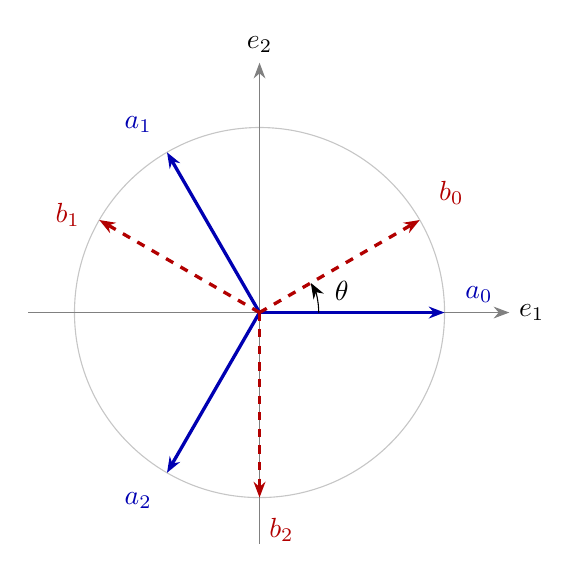
\begin{tikzpicture}[scale=2.35,>={Stealth[length=2mm,width=1.5mm]}]
  \draw[thin,gray!45] (0,0) circle (1);
  \draw[->,gray] (-1.25,0)--(1.35,0) node[right,black] {$e_1$};
  \draw[->,gray] (0,-1.25)--(0,1.35) node[above,black] {$e_2$};
  \foreach \ang/\lab/\pos in {0/{$a_0$}/{above right},120/{$a_1$}/{above left},240/{$a_2$}/{below left}}{
    \draw[blue!70!black,very thick,->] (0,0)--(\ang:1);
    \node[blue!70!black,\pos] at (\ang:1.06) {\lab};
  }
  \foreach \ang/\lab/\pos in {30/{$b_0$}/{above right},150/{$b_1$}/{left},270/{$b_2$}/{below right}}{
    \draw[red!70!black,very thick,dashed,->] (0,0)--(\ang:1);
    \node[red!70!black,\pos] at (\ang:1.06) {\lab};
  }
  \draw[thin,->] (0.32,0) arc (0:30:0.32);
  \node at (15:0.46) {$\theta$};
\end{tikzpicture}
\caption{\label{fig:mercedes}
A real size-three genuine quantum pseudocontext, drawn for
$\theta=\pi/6$.  The two triples are distinct tight frames with common
structure operator $(3/2)I_2$.}
\end{figure}

Combining these constructions with Proposition~\ref{prop:real-k2} gives the
sharp field-dependent threshold.

\begin{corollary}[Minimum genuine size]
\label{cor:threshold}
The minimum size of a genuine quantum pseudocontext is $2$ over $\C$ and $3$
over $\R$.
\end{corollary}

No size-one example exists over either field, because equality of two
rank-one projectors means equality of their rays, contradicting disjointness.

% ------------------------------------------------------------------
\section{Structure operators, Gram matrices, and Schur--Horn theory}
\label{sec:spectral}
% ------------------------------------------------------------------

Let $A:\F^k\to H$ be the synthesis operator whose columns are unit vectors
$a_1,\ldots,a_k$.  Its frame operator and Gram matrix are
\begin{equation}
 T=AA^\dagger,\qquad G=A^\dagger A
   =\bigl(\langle a_i,a_j\rangle\bigr)_{i,j=1}^{k}.
 \label{eq:frame-gram}
\end{equation}
The nonzero spectra of $T$ and $G$ agree, including multiplicities.  In
particular,
\begin{align}
 \Tr T&=k,\label{eq:trace1}\\
 \Tr(T^2)&=\sum_{i,j=1}^{k}|\langle a_i,a_j\rangle|^2
 =k+\sum_{i\ne j}|\langle a_i,a_j\rangle|^2.
 \label{eq:trace2}
\end{align}
Equation~\eqref{eq:trace2} gives another proof that a nonorthogonal family has
$\lambda_{\max}(T)>1$.

Which positive operators occur as sums of $k$ unit rank-one projectors?  The
answer is especially simple.

\begin{theorem}[Unit-norm rank-one decompositions]
\label{thm:schur-horn}
A positive operator $T$ admits a decomposition
\begin{equation}
 T=\sum_{j=1}^{k}P_{a_j},\qquad \|a_j\|=1,
 \label{eq:unit-decomposition}
\end{equation}
if and only if
\begin{equation}
 \Tr T=k,\qquad \operatorname{rank}T\le k.
 \label{eq:schur-condition}
\end{equation}
This statement allows repeated rays; distinctness is an additional condition
for quantum pseudocontexts.  The assertion holds over both $\R$ and $\C$.
\end{theorem}

\begin{proof}
Necessity is Eq.~\eqref{eq:basic-T}.  Conversely, let the positive eigenvalues
of $T$ be $\lambda_1\ge\cdots\ge\lambda_r>0$ and pad this list with $k-r$
zeros.  The resulting decreasing $k$-vector has average one, hence majorizes
$(1,\ldots,1)$: for each $m\le k$, the average of its $m$ largest
entries is at least its overall average one, and therefore
$\sum_{j=1}^{m}\lambda_j\ge m$.  By the Schur--Horn theorem
\cite{Horn-Johnson-MatrixAnalysis}, using its real symmetric version when
$\F=\R$, there is a positive semidefinite
$k\times k$ Gram matrix with this spectrum and diagonal $(1,\ldots,1)$.
Factoring the Gram matrix produces $k$ unit vectors whose frame operator has
the same nonzero eigenvalues as $T$; a unitary or orthogonal identification
of the corresponding eigenspaces then gives a decomposition of $T$ itself.
\end{proof}

Now fix a positive operator $T$ satisfying Eq.~\eqref{eq:schur-condition}.
Let $r=\operatorname{rank}T$, and let
$\lambda_1\ge\cdots\ge\lambda_r>0$ be its nonzero eigenvalues.  Fix an
orthonormal eigenbasis of $\operatorname{supp}T$ and set
$\Lambda:=\diag(\lambda_1,\ldots,\lambda_r)$.  For a decomposition
\eqref{eq:unit-decomposition}, let $M\in\F^{r\times k}$ be the coordinate
matrix of its synthesis operator in this eigenbasis.  Then
\begin{equation}
 MM^\dagger=\Lambda,\qquad \|m_j\|=1\quad(j=1,\ldots,k),
 \label{eq:canonical-fiber}
\end{equation}
where $m_j$ is its $j$th column.  Equivalently,
\begin{equation}
 M=\Lambda^{1/2}V,\qquad VV^\dagger=I_r,\qquad
 \diag(V^\dagger\Lambda V)=\1.
 \label{eq:stiefel-fiber}
\end{equation}
A quantum pseudocontext is a pair of points in this decomposition space whose
ray sets are internally distinct and mutually disjoint, modulo column phases
(signs over $\R$) and permutations.

The eigenvalues of $T$ also give the exact range of the common statistic:
\begin{equation}
 \lambda_{\min}(T)\le \Tr(\rho T)\le\lambda_{\max}(T),
 \label{eq:rayleigh}
\end{equation}
where the endpoints are attained on eigenstates.  If the ambient space is
larger than $\supp T$, then $\lambda_{\min}(T)=0$ on the full space.  On the
support, the lower endpoint is the smallest positive eigenvalue.  Every
intermediate value is obtained by a convex mixture of eigenstates associated
with the endpoint eigenvalues.

\begin{proposition}[Constancy of the common value]
\label{prop:constancy}
Let $T$ be the structure operator of a quantum pseudocontext of size $k$.
Put
\[
 S:=\supp T=\ran T,\qquad r:=\operatorname{rank}T,\qquad n:=\dim H.
\]
\begin{enumerate}
 \item The value $\Tr(\rho T)$ is constant over all density operators $\rho$
 with $\supp\rho\subseteq S$ if and only if
 \[
  T=\frac{k}{r}P_S.
 \]
 Equivalently, both families are unit-norm tight frames for $S$.
 \item The value $\Tr(\rho T)$ is constant over all density operators on $H$
 if and only if
 \[
  T=\frac{k}{n}I_H.
 \]
 In particular, this requires $r=n$.
\end{enumerate}
In case (1), the pseudocontext is genuine if and only if $k>r$.
\end{proposition}

\begin{proof}
If $T=cP_S$ and $\supp\rho\subseteq S$, then
$\Tr(\rho T)=c\Tr\rho=c$.  Taking traces gives $cr=k$, so $c=k/r$.
Conversely, suppose that $\Tr(\rho T)=c$ for every density operator supported
on $S$.  Taking $\rho=P_x$ for each unit vector $x\in S$ gives
\[
 \langle x,(T-cP_S)x\rangle=0.
\]
The self-adjoint operator $T|_S-cI_S$ therefore has vanishing quadratic form
and is zero.  Since $T$ vanishes on $S^\perp$, this gives $T=cP_S$, and the
trace again yields $c=k/r$.  This proves (1).

If $T=(k/n)I_H$, then $\Tr(\rho T)=k/n$ for every density operator on $H$.
Conversely, if this value is constant on all density operators, the same
pure-state argument on $H$ gives $T=cI_H$.  Its trace yields $c=k/n$, and
$T$ has full rank.  This proves (2).

Finally, in case (1), $\lambda_{\max}(T)=k/r$.  Proposition~\ref{prop:genuine}
therefore shows that the pseudocontext is genuine exactly when $k/r>1$, or
equivalently when $k>r$.
\end{proof}

% ------------------------------------------------------------------
\section{Symmetry and full-support real families}
\label{sec:symmetry}
% ------------------------------------------------------------------

If $U$ is unitary (orthogonal over $\R$) and commutes with $T$, then
\begin{equation}
 \sum_iP_{Ua_i}=U\left(\sum_iP_{a_i}\right)U^\dagger=T.
 \label{eq:commutant-action}
\end{equation}
Thus the isometric commutant
\begin{equation}
 \mathcal C_\F(T)=\{U:U^\dagger U=I,\ UT=TU\}
 \label{eq:commutant}
\end{equation}
acts on the decomposition space.  If the distinct eigenspaces of $T$ have
dimensions $m_\alpha$, then
\begin{equation}
 \mathcal C_\C(T)\cong\prod_\alpha U(m_\alpha),\qquad
 \mathcal C_\R(T)\cong\prod_\alpha O(m_\alpha).
 \label{eq:commutant-products}
\end{equation}
Positive spectral degeneracy therefore supplies continuous spatial freedom.
Even for a simple positive spectrum, the complex commutant contains
independent phase rotations of the one-dimensional eigenspaces, which
generically move the rays; the corresponding real commutant on the support is
discrete.

The maximally symmetric case is a distinct-ray unit-norm tight frame in
dimension $n\ge2$:
\begin{equation}
 T=\sum_{i=1}^{k}P_{a_i}=\frac{k}{n}I_n.
 \label{eq:tight-frame}
\end{equation}
Every $R\in O(n)$ preserves this operator.  Apart from the finite union of
subvarieties on which some $Ra_j$ collides with an original ray, a rotation
therefore gives a disjoint second decomposition.  If $k>n$, neither family can
be a basis, so the resulting quantum pseudocontext is genuine.

\begin{example}[Tetrahedral quantum pseudocontext]
\label{ex:tetrahedron}
In $\R^3$, let
\begin{align}
 a_1&=(0,0,1),\nonumber\\
 a_2&=\left(\frac{2\sqrt2}{3},0,-\frac13\right),\nonumber\\
 a_3&=\left(-\frac{\sqrt2}{3},\frac{\sqrt6}{3},-\frac13\right),
 \label{eq:tetrahedron}\\
 a_4&=\left(-\frac{\sqrt2}{3},-\frac{\sqrt6}{3},-\frac13\right).
 \nonumber
\end{align}
These vectors form a regular tetrahedral tight frame with
\begin{equation}
 \sum_{j=1}^{4}P_{a_j}=\frac43I_3.
 \label{eq:tetrahedron-tight}
\end{equation}
Let $R$ be the quarter-turn about the $x$ axis,
\begin{equation}
 R=\begin{pmatrix}1&0&0\\0&0&-1\\0&1&0\end{pmatrix},
 \qquad b_j=Ra_j.
 \label{eq:tetrahedron-rotation}
\end{equation}
No $b_j$ is collinear with an $a_i$, and
$\sum_jP_{b_j}=(4/3)I_3$.  The eight rays therefore form a genuine,
full-support real quantum pseudocontext of size four.
\end{example}

The same mechanism applies to any distinct-ray unit-norm tight frame in
dimension $n\ge2$: a generic collision-free orthogonal or unitary
transformation produces a disjoint second decomposition.  It does not produce
a genuine size-three example spanning
$\R^3$: if three unit vectors satisfy $\sum_{i=1}^3P_{a_i}=I_3$, then
Eq.~\eqref{eq:trace2} forces all off-diagonal inner products to vanish.  They
are an orthonormal basis.  Full-support real size-three examples must
therefore have nonscalar structure operators; concrete instances occur in
Ref.~\cite{2023-navara-svozil}.

% ------------------------------------------------------------------
\section{Operational meaning}
\label{sec:operational}
% ------------------------------------------------------------------

The projectors within one family generally do not commute and cannot be
measured together as one sharp test.  The statistic
\begin{equation}
 \rho\longmapsto\sum_i\Tr(\rho P_{a_i})=\Tr(\rho T)
 \label{eq:linear-statistic}
\end{equation}
is estimated from separate compatible measurement arrangements on repeated
preparations.  Its equivalence with the $b$-statistic is exact for every
quantum state.

The same identity has a preparation-side reading.  By
Eq.~\eqref{eq:basic-T},
\begin{equation}
 \rho_T:=\frac{T}{k}
 =\frac1k\sum_{i=1}^{k}P_{a_i}
 =\frac1k\sum_{i=1}^{k}P_{b_i}
 \label{eq:uniform-ensembles}
\end{equation}
is a density operator.  Thus a quantum pseudocontext also specifies two
ray-disjoint, equal-cardinality, uniformly weighted pure-state ensembles with
the same average state.  Over $\C$, this is a constrained instance of the
Hughston--Jozsa--Wootters classification of pure-state ensembles of a fixed
density operator~\cite{Hughston-Jozsa-Wootters-1993}: here the two
decompositions additionally have the same cardinality and uniform weights,
and their ray sets are disjoint.  Once the preparation label is discarded,
no quantum measurement on the system alone can distinguish which of the two
randomization procedures produced it, although their labelled fine-grained
data remain different.

There is also a direct positive operator-valued measure (POVM) formulation.
Since $0\le T\le kI$, the effects
\begin{align}
 E_i&=\frac1kP_{a_i},&E_0&=I-\frac1kT,\nonumber\\
 F_i&=\frac1kP_{b_i},&F_0&=I-\frac1kT
 \label{eq:povms}
\end{align}
define two POVMs.  Their non-residual outcomes have the same coarse-grained
effect $T/k$.  If $T=(k/r)I$ on an $r$-dimensional support, the more natural
normalization $(r/k)P_{a_i}$ removes the residual effect on that support and
gives two rank-one tight-frame POVMs.

Equations~\eqref{eq:uniform-ensembles} and \eqref{eq:povms} are dual
operational uses of the same projector identity: it generates a preparation
equivalence after randomization and a measurement equivalence after
coarse-graining.  Neither statement identifies the individual labelled
preparations or outcomes.

State-independence also supplies a null consistency test.  For two laboratory
implementations intended to realize the displayed ray families, the signed
difference
\begin{equation}
 \Delta(\rho):=
 \sum_i\Tr(\rho P_{a_i})-\sum_i\Tr(\rho P_{b_i})
 \label{eq:null-test}
\end{equation}
must vanish for every fixed, otherwise unknown input state.  Comparing the
two empirical sums therefore requires neither state tomography nor prior
knowledge of $\rho$.  A statistically significant nonzero value diagnoses a
failure among the assumed projectors, relative detector responses, source
stationarity, or the quantum model; by itself it neither localizes the fault
nor certifies nonclassicality.

There is an analogous decomposition-level consequence outside the immediate
measurement setting.  If $T$ is regarded as a positive Hamiltonian written
as a sum of rank-one terms, the two ray families give disjoint term lists
with exactly the same Hamiltonian and hence the same spectrum and time
evolution.  Additional implementation constraints, such as locality, may
make one list preferable, but observations of $T$ alone cannot identify
which decomposition was used.

This equivalence is related to, but is not by itself, generalized
contextuality in the sense of Spekkens~\cite{Spekkens-04}.  Nor is it a
Kochen--Specker contradiction.  The four-ray assignment
\eqref{eq:classical-counterexample} demonstrates that an ontological or
classical model is under no obligation to respect the quantum identity unless
the equality is added as an operational equivalence or follows independently
from its own admissibility constraints.

% ------------------------------------------------------------------
\section{Relation to hypergraph-forced pseudocontexts}
\label{sec:relation}
% ------------------------------------------------------------------

In standard graph-theoretic terminology, a \emph{faithful orthogonal
representation} (FOR), also called a faithful coordinatization, assigns
distinct rays to the vertices so that two rays are orthogonal exactly when
the corresponding vertices share a hyperedge
\cite{lovasz-79,lovasz-89,Portillo-2015}.  More precisely, suppose that the
equality of two probability sums is obtained as a balanced linear combination
of full-context normalization equations.  Under a FOR, every full context is
represented by an orthonormal basis and its projectors resolve the identity.
Applying the same balanced linear combination to these projector resolutions
yields the corresponding projector-sum equality.  Thus every
hypergraph-forced pseudocontext in this sense whose hypergraph admits a FOR
yields a quantum pseudocontext.  The converse fails for the induced bare
orthogonality hypergraph: a projector identity need not follow from its own
orthogonality relations.  Example~\ref{ex:k2} has no bare context equations,
and a generic tight frame paired with a generic rotation also carries too
little bare orthogonality data to imply its projector-sum identity.

Whether a given identity can be forced after adjoining finitely many
auxiliary vertices and contexts is a separate completion problem, not part
of Definition~\ref{def:quantum-pseudocontext}.  A complex three-dimensional
size-two completion and its field-dependent realizability are studied in
Ref.~\cite{2026-Navara-Svozil-complex-only-3d-hypergraphs}; the general
finite-completion question remains open.

% ------------------------------------------------------------------
\section{Open problems}
% ------------------------------------------------------------------

\begin{problem}[Decomposition moduli]
For a fixed positive $T$, determine the connected components and singular
strata of the unit-norm decomposition space in
Eq.~\eqref{eq:canonical-fiber}, modulo column phases, permutations, and the
isometric commutant of $T$.
\end{problem}

\begin{problem}[Disjoint decomposition criterion]
Strengthen Theorem~\ref{thm:schur-horn} from the existence of one unit-norm
decomposition to a spectral or geometric criterion for two ray-disjoint
decompositions, over both $\R$ and $\C$.
\end{problem}

\begin{problem}[Finite forcing completion]
Characterize those quantum pseudocontexts that admit a finite auxiliary
context hypergraph whose normalization equations force their equality.  In
particular, determine which generic tight-frame rotations have such a
completion.
\end{problem}

% ------------------------------------------------------------------
\section{Conclusion}
% ------------------------------------------------------------------

Quantum pseudocontexts are pairs of disjoint unit-norm rank-one
decompositions of one positive operator.  Dividing that operator by the
common family size gives two uniform pure-state ensembles of one density
operator; normalizing the summands as effects gives two POVMs with a common
coarse-graining.  Their defining equality holds for all density operators
because quantum states separate self-adjoint operators.
This universality is internal to the chosen quantum coordinatization: it does
not make the equality a consequence of a bare orthogonality hypergraph and
does not constrain arbitrary classical or softmax probabilities.

The distinction exposes a clean mathematical structure.  In $\C^2$, equal
projector sums are equal Bloch centroids; complex phase freedom permits
genuine examples of size two, while real doubled-angle geometry excludes
genuine examples of that size.  Schur--Horn theory
describes the possible structure operators, their canonical fibers describe
all unit-norm decompositions, and spectral degeneracy generates continuous
families through the commutant.  These operator-level identities are useful
as quantum equivalences in their own right, independently of whether any
finite hypergraph can force them.



\begin{acknowledgments}
During manuscript preparation, the authors used OpenAI Codex (GPT-5) to assist with literature organization, LaTeX editing, exact symbolic checks, and figure/PDF verification; all AI-assisted output was directed and critically reviewed by the authors, who independently verified the mathematics and take full responsibility for the final content, and no AI tool is an author.
This research was funded in part by the Austrian
Science Fund (FWF), Grant DOI \href{https://doi.org/10.55776/PIN5424624}{10.55776/PIN5424624}, and the Czech Science
Foundation (GA\v{C}R), Grant No.~25-20013L.  The authors declare no
conflict of interest.
\end{acknowledgments}

\bibliography{svozil}

\end{document}
